\subsection{Szelektorok}

%7
\begin{frame}
  \begin{description}[m]
    \item[HTML elem neve] \hfill \\ \texttt{p \{ font-style: italic; \}}
    \item[Egyedi azonosító (\texttt{id} attribútum) alapján] \hfill \\ 
      \texttt{\#lablec \{ font-size: 10pt; \}}\\
      Az \texttt{id} nem kezdődhet számjegy karakterrel!
    \item[Univerzális szelektor, mindenre illeszkedik] \hfill \\ \texttt{* \{ font-size: smaller; \}}
  \end{description}
\end{frame}

%8
\begin{frame}
  \begin{description}[m]
    \item[Osztály (\texttt{class} attribútum alapján)] \hfill \\ 
      \texttt{*.kisbetus \{ font-size: small; \} /* bármilyen HTML elemhez */} \\
      \texttt{.kisbetus \{ font-size: small; \} /* bármilyen HTML elemhez, rövid alak */}\\
      \texttt{p.voros \{ color: red; \} /* csak adott (pl. <p>) HTML elemhez */}\\
      A \texttt{class} értéke nem kezdődhet számjeggyel, de lehet egyszerre több, szóközzel elválasztott értéke: \\
      \texttt{<p class="kisbetus voros">Apróbetűs piros bekezdés</p>}
    \item[Elemek csoportosítása] \hfill \\ \texttt{h1, h2, h3 \{ font-family: Arial; \}}
  \end{description}
\end{frame}

%9
\begin{frame}
  \begin{exampleblock}{\textattachfile{egyszeruSzelektor1.html}{egyszeruSzelektor1.html}}
    \scriptsize
    \lstinputlisting[style=HTML,linerange={3-13},numbers=left,firstnumber=3]{egyszeruSzelektor1.html}
  \end{exampleblock}
\end{frame}

%10
\begin{frame}
  \begin{exampleblock}{\textattachfile{egyszeruSzelektor1.html}{egyszeruSzelektor1.html}}
    \scriptsize
    \lstinputlisting[style=HTML,linerange={14-15},numbers=left,firstnumber=14]{egyszeruSzelektor1.html}
  \end{exampleblock}
\end{frame}

%11
\begin{frame}
  \begin{exampleblock}{\textattachfile{egyszeruSzelektor1.css}{egyszeruSzelektor1.css}}
    \scriptsize
    \lstinputlisting[style=HTML,numbers=left]{egyszeruSzelektor1.css}
  \end{exampleblock}
  \begin{center}
    
\includegraphics[width=.9\textwidth]{egyszeruSzelektor1.png}
  \end{center}
\end{frame}

%_
\begin{frame}
  Egy elembe tetszőleges mélységben beágyazott másik elemek kiválasztása
  \begin{columns}[c]
    \column{0.66\textwidth}
      \begin{exampleblock}{\textattachfile{leszarmazott.html}{leszarmazott.html}}
        \footnotesize
        \lstinputlisting[style=HTML,linerange={7-7},numbers=left,firstnumber=7]{leszarmazott.html}
        \lstinputlisting[style=HTML,linerange={11-18},numbers=left,firstnumber=11]{leszarmazott.html}
      \end{exampleblock}
    \column{0.3\textwidth}
      
\includegraphics[width=\textwidth]{leszarmazott.png}
  \end{columns}
\end{frame}

%_
\begin{frame}
  Egy elembe közvetlenül beágyazott gyermek elemek kiválasztása
  \begin{columns}[c]
    \column{0.66\textwidth}
      \begin{exampleblock}{\textattachfile{gyermek.html}{gyermek.html}}
        \footnotesize
        \lstinputlisting[style=HTML,linerange={7-7},numbers=left,firstnumber=7]{gyermek.html}
        \lstinputlisting[style=HTML,linerange={11-18},numbers=left,firstnumber=11]{gyermek.html}
      \end{exampleblock}
    \column{0.3\textwidth}
      
\includegraphics[width=\textwidth]{gyermek.png}
  \end{columns}
\end{frame}

%_
\begin{frame}
  Egy elemet közvetlenül követő testvér elem kiválasztása
  \begin{columns}[c]
    \column{0.66\textwidth}
      \begin{exampleblock}{\textattachfile{testver.html}{testver.html}}
        \footnotesize
        \lstinputlisting[style=HTML,linerange={7-7},numbers=left,firstnumber=7]{testver.html}
        \lstinputlisting[style=HTML,linerange={11-19},numbers=left,firstnumber=11]{testver.html}
      \end{exampleblock}
    \column{0.3\textwidth}
      
\includegraphics[width=\textwidth]{testver.png}
  \end{columns}
\end{frame}

%_
\begin{frame}
  Egy elemet közvetlenül követő összes testvér kiválasztása
  \begin{columns}[c]
    \column{0.66\textwidth}
      \begin{exampleblock}{\textattachfile{testver2.html}{testver2.html}}
        \footnotesize
        \lstinputlisting[style=HTML,linerange={7-7},numbers=left,firstnumber=7]{testver2.html}
        \lstinputlisting[style=HTML,linerange={11-19},numbers=left,firstnumber=11]{testver2.html}
      \end{exampleblock}
    \column{0.3\textwidth}
      
\includegraphics[width=\textwidth]{testver2.png}
  \end{columns}
\end{frame}

%_
\begin{frame}
  Látszólagos osztályok (pseudo-class): egy elem adott állapota esetén alkalmazandó formázása, 
  \hiv{\href{https://developer.mozilla.org/en-US/docs/Web/CSS/Pseudo-classes}{referencia}}
  \vfill
  Az egér alatti elem kiválasztása
  \begin{columns}[c]
    \column{0.66\textwidth}
      \begin{exampleblock}{\textattachfile{hover.html}{hover.html}}
        \footnotesize
        \lstinputlisting[style=HTML,linerange={7-7},numbers=left,firstnumber=7]{hover.html}
        \lstinputlisting[style=HTML,linerange={11-11},numbers=left,firstnumber=11]{hover.html}
      \end{exampleblock}
    \column{0.3\textwidth}
      
\includegraphics[width=\textwidth]{hover1.png}
      \vfill
      
\includegraphics[width=\textwidth]{hover2.png}
  \end{columns}
\end{frame}

%_
\begin{frame}
  Azon elemek kiválasztása, melyek a szülőjük első gyermekei
  \begin{columns}[c]
    \column{0.66\textwidth}
      \begin{exampleblock}{\textattachfile{firstchild.html}{firstchild.html}}
        \scriptsize
        \lstinputlisting[style=HTML,linerange={7-7},numbers=left,firstnumber=7]{firstchild.html}
        \lstinputlisting[style=HTML,linerange={10-14},numbers=left,firstnumber=10]{firstchild.html}
      \end{exampleblock}
    \column{0.3\textwidth}
      
\includegraphics[width=\textwidth]{firstchild.png}
  \end{columns}
\end{frame}

%_
\begin{frame}
  Nyelvfüggő beállítások alkalmazása
  \begin{columns}[c]
    \column{0.66\textwidth}
      \begin{exampleblock}{\textattachfile{lang.html}{lang.html}}
        \scriptsize
        \lstinputlisting[style=HTML,linerange={7-7},numbers=left,firstnumber=7]{lang.html}
        \lstinputlisting[style=HTML,linerange={11-12},numbers=left,firstnumber=11]{lang.html}
      \end{exampleblock}
    \column{0.3\textwidth}
      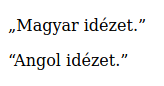
\includegraphics[width=\textwidth]{lang.png}
  \end{columns}
\end{frame}

%_
\begin{frame}
  Adott típus n-edik előfordulása (részleteket ld. később \texttt{nth-child()}-nál)
  \begin{columns}[c]
    \column{0.7\textwidth}
      \begin{exampleblock}{\textattachfile{nthoftype.html}{nthoftype.html}}
        \scriptsize
        \lstinputlisting[style=HTML,linerange={7-7},numbers=left,firstnumber=7]{nthoftype.html}
        \lstinputlisting[style=HTML,linerange={11-16},numbers=left,firstnumber=11]{nthoftype.html}
      \end{exampleblock}
    \column{0.25\textwidth}
      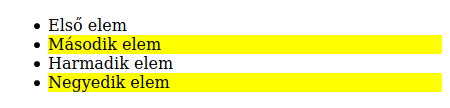
\includegraphics[width=\textwidth]{nthoftype.png}
  \end{columns}
\end{frame}

%_
\begin{frame}
  Látszólagos elemek (pseudo-elements): elemek bizonyos részeinek kiválasztása
  \vfill
  Első sor kiválasztása: \texttt{::first-line}
  \begin{itemize}
    \item Csak blokkszintű elemekkel használható
    \item Csak bizonyos tulajdonságokkal használható: \\ \tiny \texttt{font}, \texttt{word-spacing}, \texttt{letter-spacing}, \texttt{line-height}, \texttt{text-decoration}, \texttt{text-transform}, \texttt{vertical-align}, \texttt{color}, \texttt{background}, \texttt{clear}.
  \end{itemize}
  \vfill
  CSS3 előtt \kiemel{:} állt ott, ahol most \kiemel{::}.
\end{frame}

%_
\begin{frame}
  Szöveg első betűjének kiválasztása: \texttt{::first-letter}
  \begin{itemize}
    \item Csak blokkszintű elemekkel használható
    \item Csak bizonyos tulajdonságokkal használható: \\ \tiny \texttt{font}, \texttt{line-height}, \texttt{text-decoration}, \texttt{text-transform}, \texttt{color}, \texttt{background}, \texttt{margin}, \texttt{border}, \texttt{padding}, \texttt{vertical-align} (ha nincs lebegtetés), \texttt{float}, \texttt{clear}.
  \end{itemize}
  \vfill
  Kijelölt szöveg: \texttt{::selection}
    \begin{itemize}
    \item Csak bizonyos tulajdonságokkal használható: \\ \tiny \texttt{color}, \texttt{background}, \texttt{cursor}, \texttt{outline}.
  \end{itemize}
\end{frame}

%_
\begin{frame}
  Tartalom valami előtt: \texttt{::before}, mögött: \texttt{::after}\\
  \vfill
  Tartalom megadása: \texttt{content} tulajdonsággal, értéke:
  \begin{itemize}
    \item idézőjelek/aposztrófok közötti szöveg
    \item karakterek unicode kódja, pl. \texttt{'\textbackslash 02192'} $\equiv ~ \to$
    \item \texttt{url()} függvénnyel adott kép
  \end{itemize}
\end{frame}

%_
\begin{frame}
  \begin{columns}[T]
    \column{0.4\textwidth}
      \begin{exampleblock}{\textattachfile{pseudoelements.html}{pseudoelements.html}}
        \fontsize{7}{8} \selectfont
        \lstinputlisting[style=HTML,linerange={7-14},numbers=left,firstnumber=7]{pseudoelements.html}
      \end{exampleblock}
    \column{0.52\textwidth}
      \begin{exampleblock}{}
        \fontsize{7}{8} \selectfont
        \lstinputlisting[style=HTML,linerange={15-26},numbers=right,firstnumber=15]{pseudoelements.html}
      \end{exampleblock}
  \end{columns}
  \begin{exampleblock}{}
    \fontsize{7}{8} \selectfont
    \vspace{-0.1cm}
    \lstinputlisting[style=HTML,linerange={30-34},numbers=left,firstnumber=30]{pseudoelements.html}
    \vspace{-0.1cm}
  \end{exampleblock}
\end{frame}

%_
\begin{frame}
  \begin{center}
    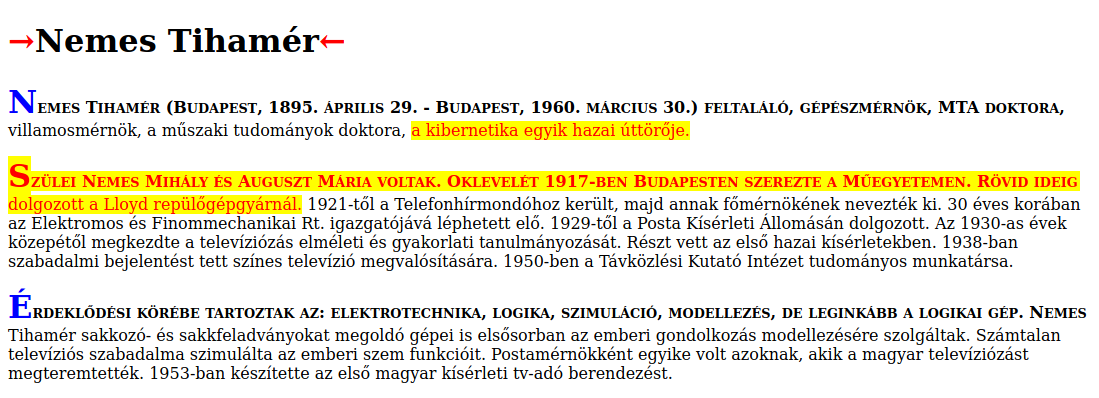
\includegraphics[width=\textwidth]{pseudoelements.png}\\
    \textattachfile{pseudoelements.html}{pseudoelements.html}
  \end{center}
\end{frame}

%_
\begin{frame}
  Kiválasztás attribútumok alapján
  \vfill
  Adott attribútummal rendelkező elemek kiválasztása
  \begin{exampleblock}{\textattachfile{attributum1.html}{attributum1.html}}
    \fontsize{7}{8} \selectfont
    \lstinputlisting[style=HTML,linerange={7-7},numbers=left,firstnumber=7]{attributum1.html}
    \lstinputlisting[style=HTML,linerange={12-13},numbers=left,firstnumber=12]{attributum1.html}
  \end{exampleblock}
  \begin{center}
    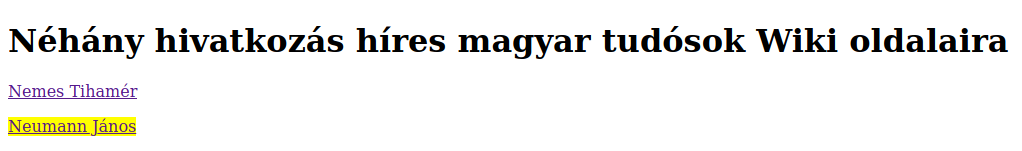
\includegraphics[width=0.6\textwidth]{attributum1.png}
  \end{center}
\end{frame}

%_
\begin{frame}
  Pontosan az adott értékű attribútummal rendelkező elemek kiválasztása
  \begin{exampleblock}{\textattachfile{attributum2.html}{attributum2.html}}
    \fontsize{7}{8} \selectfont
    \lstinputlisting[style=HTML,linerange={7-7},numbers=left,firstnumber=7]{attributum2.html}
    \lstinputlisting[style=HTML,linerange={12-13},numbers=left,firstnumber=12]{attributum2.html}
  \end{exampleblock}
  \begin{center}
    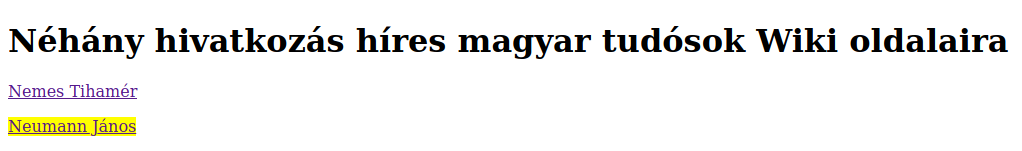
\includegraphics[width=0.6\textwidth]{attributum2.png}
  \end{center}
\end{frame}

%_
\begin{frame}
  Adott teljes szót (is) tartalmazó értékű attribútummal rendelkező elemek kiválasztása
  \begin{columns}[c]
    \column{0.7\textwidth}
      \begin{exampleblock}{\textattachfile{attributum3.html}{attributum3.html}}
      \scriptsize
      \lstinputlisting[style=HTML,linerange={7-7},numbers=left,firstnumber=7]{attributum3.html}
      \lstinputlisting[style=HTML,linerange={12-14},numbers=left,firstnumber=12]{attributum3.html}
  \end{exampleblock}
    \column{0.27\textwidth}
      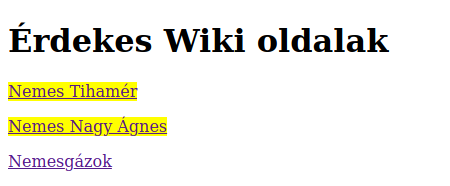
\includegraphics[width=\textwidth]{attributum3.png}
  \end{columns}
\end{frame}

%_
\begin{frame}
  Kiválasztja az elemet, ha az adott attribútumnak a megadott szó az egyetlen értéke, esetleg ezzel kezdődik és kötőjellel folytatódik
  \begin{columns}[c]
    \column{0.7\textwidth}
      \begin{exampleblock}{\textattachfile{attributum4.html}{attributum4.html}}
      \fontsize{7}{8} \selectfont
      \lstinputlisting[style=HTML,linerange={7-7},numbers=left,firstnumber=7]{attributum4.html}
      \lstinputlisting[style=HTML,linerange={12-16},numbers=left,firstnumber=12]{attributum4.html}
  \end{exampleblock}
    \column{0.27\textwidth}
      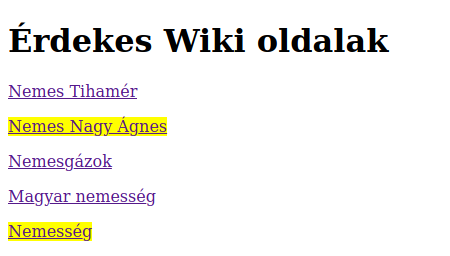
\includegraphics[width=\textwidth]{attributum4.png}
  \end{columns}
\end{frame}

%_
\begin{frame}
  Kiválasztja az elemet, ha attribútumának értéke az adott karaktersorozattal kezdődik
  \begin{columns}[c]
    \column{0.7\textwidth}
      \begin{exampleblock}{\textattachfile{attributum5.html}{attributum5.html}}
      \fontsize{7}{8} \selectfont
      \lstinputlisting[style=HTML,linerange={7-7},numbers=left,firstnumber=7]{attributum5.html}
      \lstinputlisting[style=HTML,linerange={12-16},numbers=left,firstnumber=12]{attributum5.html}
  \end{exampleblock}
    \column{0.27\textwidth}
      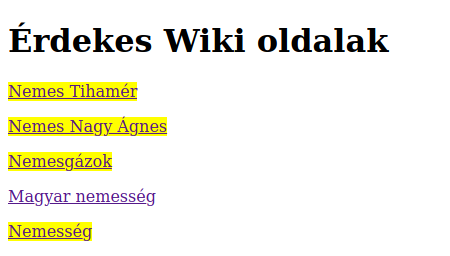
\includegraphics[width=\textwidth]{attributum5.png}
  \end{columns}
\end{frame}

%_
\begin{frame}
  Kiválasztja az elemet, ha attribútumának értéke az adott karaktersorozattal fejeződik be
  \begin{columns}[c]
    \column{0.7\textwidth}
      \begin{exampleblock}{\textattachfile{attributum6.html}{attributum6.html}}
      \fontsize{7}{8} \selectfont
      \lstinputlisting[style=HTML,linerange={7-7},numbers=left,firstnumber=7]{attributum6.html}
      \lstinputlisting[style=HTML,linerange={12-16},numbers=left,firstnumber=12]{attributum6.html}
  \end{exampleblock}
    \column{0.27\textwidth}
      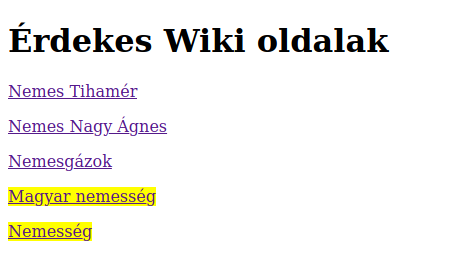
\includegraphics[width=\textwidth]{attributum6.png}
  \end{columns}
\end{frame}

%_
\begin{frame}
  Kiválasztja az elemet, ha attribútumának értéke tartalmazza az adott karaktersorozatot
  \begin{columns}[c]
    \column{0.7\textwidth}
      \begin{exampleblock}{\textattachfile{attributum7.html}{attributum7.html}}
      \fontsize{7}{8} \selectfont
      \lstinputlisting[style=HTML,linerange={7-7},numbers=left,firstnumber=7]{attributum7.html}
      \lstinputlisting[style=HTML,linerange={12-16},numbers=left,firstnumber=12]{attributum7.html}
  \end{exampleblock}
    \column{0.27\textwidth}
      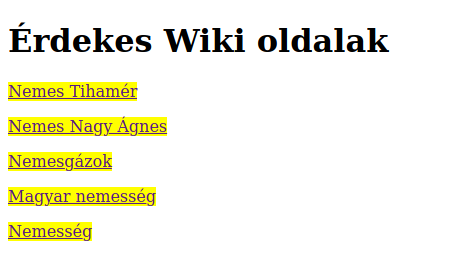
\includegraphics[width=\textwidth]{attributum7.png}
  \end{columns}
\end{frame}
